\subsection{Roles}

Para llevar a cabo la creación de los distintos roles se debe estar en la perspectiva avanzada de TIBCO EBX. Posteriormente, en el apartado de “Administración” (Llave inglesa) se debe acceder a “Directorio”, donde se encontrará la opción de “Roles”.

\begin{figure}[H]
    \centering
    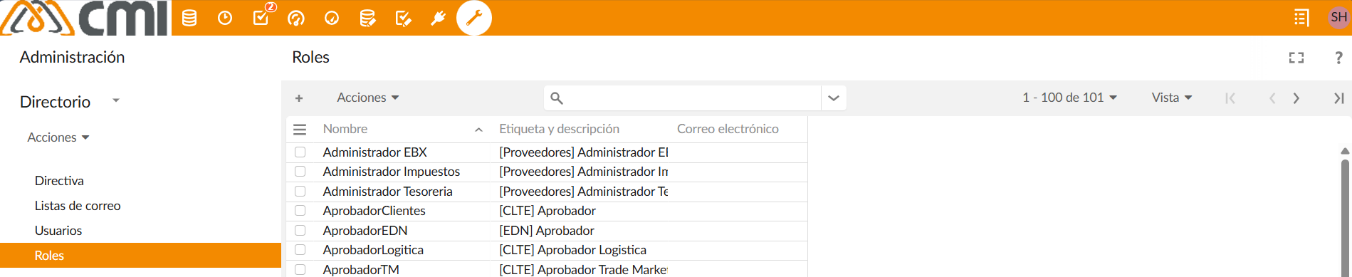
\includegraphics[width=0.8\textwidth]{RolesUsuario/ImgRolesUsuario/RS01.png}
    \caption{Directorio de Roles dentro de Administración.}
\end{figure}

Se dará clic en el símbolo de más (+) para crear un nuevo rol. 

\begin{figure}[H]
    \centering
    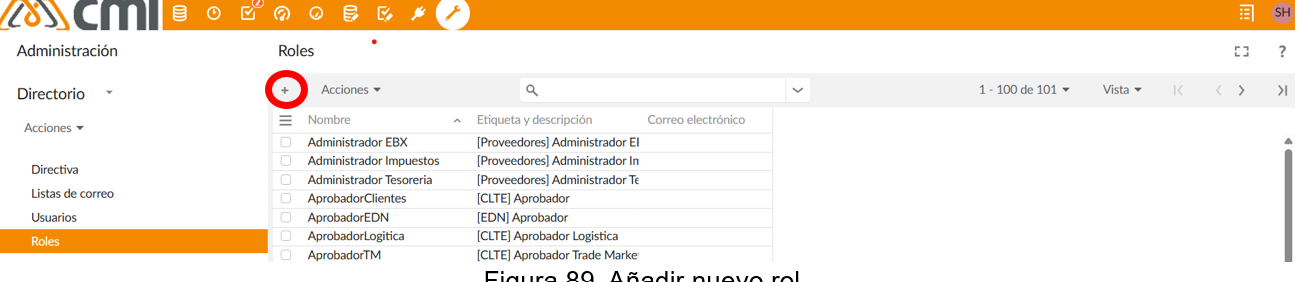
\includegraphics[width=0.8\textwidth]{RolesUsuario/ImgRolesUsuario/RS02.png}
    \caption{Añadir nuevo rol}
\end{figure}

Se abrirá un nuevo apartado donde se asignará el nombre del nuevo rol, así como una descripción de éste.   

\begin{figure}[H]
    \centering
    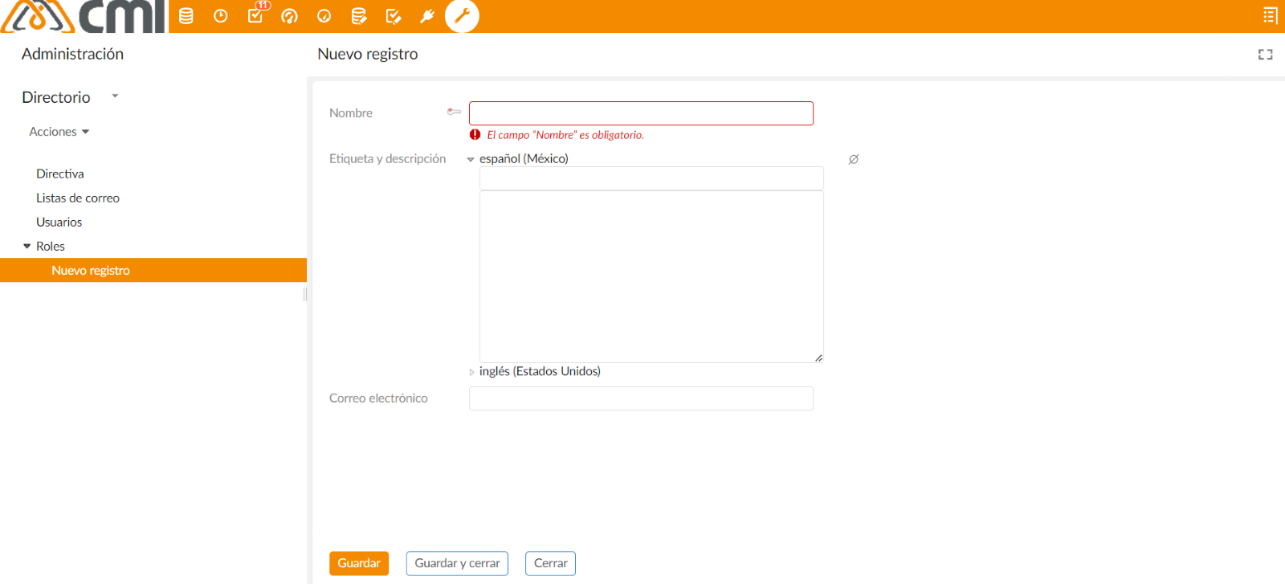
\includegraphics[width=0.8\textwidth]{RolesUsuario/ImgRolesUsuario/RS03.png}
    \caption{Registro de nuevo rol.}
\end{figure}

Una vez llenados los distintos apartados, se dará clic en “guardar y cerrar” y de esta manera quedará creado el nuevo rol.  

Al momento se tienen creados 29 roles para el proceso de Cuentas Contables:

\begin{itemize}

    \item [[EBX] Técnico Administrador]
    \item [[I] Integraciones]
    \item [[CuCo] Solicitante]
    \item [[CuCo] Validador Datos Maestros]
    \item [[CuCo] Validador Datos Maestros (400)]
    \item [[CuCo] Validador Datos Maestros (401)]
    \item [[CuCo] Validador Datos Maestros (402)]
    \item [[CuCo] Validador Datos Maestros (404)]
    \item [[CuCo] Validador Datos Maestros (406)]
    \item [[CuCo] Validador Datos Maestros (420)]
    \item [[CuCo] Validador Datos Maestros (510)]
    \item [[CuCo] Validador de NEFI]
    \item [[CuCo] Validador de NEFI (400)]
    \item [[CuCo] Validador de NEFI (401)]
    \item [[CuCo] Validador de NEFI (402)]
    \item [[CuCo] Validador de NEFI (404)]
    \item [[CuCo] Validador de NEFI (406)]
    \item [[CuCo] Validador de NEFI (420)]
    \item [[CuCo] Validador de NEFI (510)]
    \item [[CuCo] Solicitante - Colombia]
    \item [[CuCo] Solicitante - Guatemala]
    \item [[CuCo] Solicitante - Honduras]
    \item [[CuCo] Solicitante - México]
    \item [[CuCo] Solicitante - Nicaragua]
    \item [[CuCo] Solicitante - Panamá]
    \item [[CuCo] Solicitante - Costa Rica]
    \item [[CuCo] Solicitante - El Salvador]
    \item [[CuCo] Solicitante - Estados Unidos]
    \item [[CuCo] Solicitante - República Dominicana]
    \item [[CuCo] Histórico]

\end{itemize}